\documentclass{article}
\usepackage[utf8]{inputenc}
\usepackage[english]{babel}
\usepackage[obeyspaces]{url}
\usepackage{amsfonts}
\usepackage{amsmath}
\usepackage{amssymb}
\usepackage{hyperref}
\usepackage{adjustbox}
\usepackage{tikz}
\usetikzlibrary{calc,matrix,positioning,arrows.meta,arrows}

\tikzset{
mymat/.style={
  matrix of math nodes,
  text height=2.5ex,
  text depth=0.75ex,
  text width=3.25ex,
  align=center,
  column sep=-\pgflinewidth
  },
mymats/.style={
  mymat,
  nodes={draw,fill=#1},
  }  
}

\title{
    Introduction to Algorithms\\3rd Edition\\---\\
    Thomas H. Cormen, Charles E. Leiserson, Ronald L. Rivest, \& Clifford Stein
}
\author{Graham Strickland}

\begin{document}
\maketitle  

\section{The Role of Algorithms in Computing}
% Chapter 2

\subsection*{2.1 Insertion sort}
% Section 2.1

\subsubsection*{2.1-1}
\begin{itemize}
    \item[(a)]
        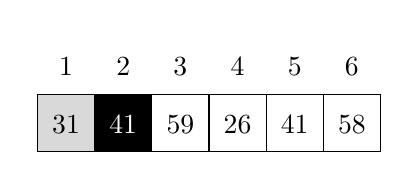
\begin{tikzpicture}[>=latex]
            \tikzstyle{row 2 column 1} = [nodes={fill=gray!30}]
            \tikzstyle{row 2 column 2} = [nodes={fill=black},text=white]
            \matrix[mymat,anchor=west,row 2/.style={nodes=draw}]
            {
                1  & 2  & 3  & 4  & 5  & 6 \\
                31 & 41 & 59 & 26 & 41 & 58 \\
            };
        \end{tikzpicture}
    \item[(b)]
        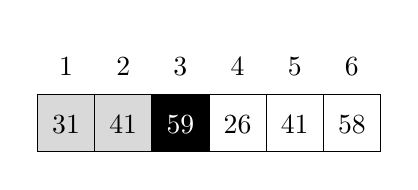
\begin{tikzpicture}[>=latex]
            \tikzstyle{row 2 column 1} = [nodes={fill=gray!30}]
            \tikzstyle{row 2 column 2} = [nodes={fill=gray!30}]
            \tikzstyle{row 2 column 3} = [nodes={fill=black},text=white]
            \matrix[mymat,anchor=west,row 2/.style={nodes=draw}]
            {
                1  & 2  & 3  & 4  & 5  & 6 \\
                31 & 41 & 59 & 26 & 41 & 58 \\
            };
        \end{tikzpicture}
    \item[(c)]
        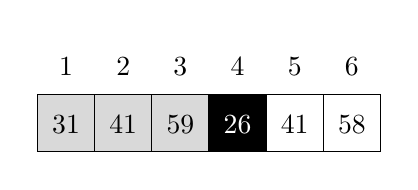
\begin{tikzpicture}[>=latex]
            \tikzstyle{row 2 column 1} = [nodes={fill=gray!30}]
            \tikzstyle{row 2 column 2} = [nodes={fill=gray!30}]
            \tikzstyle{row 2 column 3} = [nodes={fill=gray!30}]
            \tikzstyle{row 2 column 4} = [nodes={fill=black},text=white]
            \matrix[mymat,anchor=west,row 2/.style={nodes=draw}]
            {
                1  & 2  & 3  & 4  & 5  & 6 \\
                31 & 41 & 59 & 26 & 41 & 58 \\
            };
        \end{tikzpicture}
    \item[(d)]
        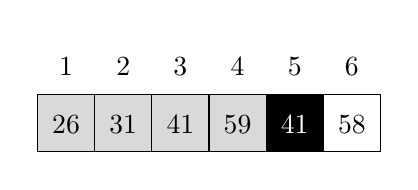
\begin{tikzpicture}[>=latex]
            \tikzstyle{row 2 column 1} = [nodes={fill=gray!30}]
            \tikzstyle{row 2 column 2} = [nodes={fill=gray!30}]
            \tikzstyle{row 2 column 3} = [nodes={fill=gray!30}]
            \tikzstyle{row 2 column 4} = [nodes={fill=gray!30}]
            \tikzstyle{row 2 column 5} = [nodes={fill=black},text=white]
            \matrix[mymat,anchor=west,row 2/.style={nodes=draw}]
            {
                1  & 2  & 3  & 4  & 5  & 6 \\
                26 & 31 & 41 & 59 & 41 & 58 \\
            };
        \end{tikzpicture}
    \item[(e)]
        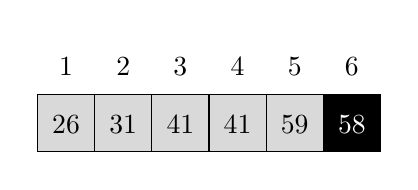
\begin{tikzpicture}[>=latex]
            \tikzstyle{row 2 column 1} = [nodes={fill=gray!30}]
            \tikzstyle{row 2 column 2} = [nodes={fill=gray!30}]
            \tikzstyle{row 2 column 3} = [nodes={fill=gray!30}]
            \tikzstyle{row 2 column 4} = [nodes={fill=gray!30}]
            \tikzstyle{row 2 column 5} = [nodes={fill=gray!30}]
            \tikzstyle{row 2 column 6} = [nodes={fill=black},text=white]
            \matrix[mymat,anchor=west,row 2/.style={nodes=draw}]
            at (0,0)
            (mat1)
            {
                1  & 2  & 3  & 4  & 5  & 6 \\
                26 & 31 & 41 & 41 & 59 & 58 \\
            };
        \end{tikzpicture}
    \item[(f)]
        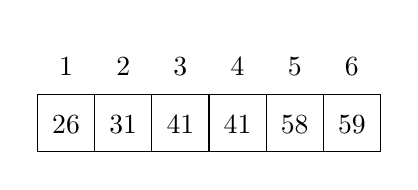
\begin{tikzpicture}[>=latex]
            \matrix[mymat,anchor=west,row 2/.style={nodes=draw}]
            at (0,0)
            (mat1)
            {
                1  & 2  & 3  & 4  & 5  & 6 \\
                26 & 31 & 41 & 41 & 58 & 59 \\
            };
        \end{tikzpicture}
\end{itemize}


\subsubsection*{2.1-2}
% Exercise 2.1-2

\begin{algorithmic}[1]
    \TITLE{\textsc{Insertion-Sort}$(A)$}
    \FOR{$j = 2$ \TO $A.\mathit{length}$}
            \STATE $\mathit{key} = A[j]$
            \STATE \COMMENT{Insert $A[j]$ to the sorted sequence $A[1\, .\, .\, j - 1]$}
            \STATE $i = j-1$
        \WHILE{$i>0$ \AND $A[i] < key$}
            \STATE $A[i+1]= A[i]$
            \STATE $i = i-1$
        \ENDWHILE
            \STATE $A[i+1] = \mathit{key}$
    \ENDFOR
\end{algorithmic}

The implementation can be seen in the following file:

\path{rs/clrs_algorithms/src/sorting.rs}.


\subsubsection*{2.1-3}
% Exercise 2.1-3

\begin{algorithmic}[1]
    \TITLE{\textsc{Linear-Search}$(A, \nu)$}
    \STATE $j = 1$
    \WHILE{$j \neq A.\mathit{length}$}
        \IF{$A[j] == \nu$}
            \RETURN $j$
        \ELSE
            \STATE $j = j + 1$
        \ENDIF
    \ENDWHILE
    \RETURN \textrm{NIL}
\end{algorithmic}

\begin{description}
    \item[Initialization:] With the loop invariant being that $A[j]$ refers to an 
        element of the sequence $A = \langle a_1, a_2, \ldots, a_n \rangle$ and 
        each element in $A[1\, .\, .\, j - 1]$ has been checked for equality, we 
        have the loop invariant valid, since $j = 1$ and $A[1]$ is in $A$ for 
        $n \ge 1$, at the start of the \textbf{while} loop 1 -- 6.
    \item[Maintenance:] Either the \textbf{if} statement in line 3 returns $A[j]$
        or the \textbf{else} statement in line 5 increments $j$ by 1, so that after
        each pass of the \textbf{while} loop, we have checked whether or not 
        $A[j] = \nu$, and the condition of the \textbf{while} loop ensures that 
        $A[j]$ is in $A$.
    \item[Termination:] If the \textbf{while} loop terminates, then either the 
        \textbf{if} condition in line 3 is true, so that $A[j] = \nu$ or 
        $j = A.\mathit{length}$, at which point we return the special value
        \textrm{NIL}.
\end{description}

Thus the algorithm is correct, since the loop invariant is initialized and 
maintained throughout, and the algorithm terminates with the correct output;
if a value is returned, $\nu$ is in $A$, and occurs at $A[j]$ for return value
$j$, otherwise the special value \textrm{NIL} was returned, and $\nu$ is not in $A$.

The implementation can be seen in the following file:

\path{src/algorithms/search/linear_search.h}.


\subsubsection*{2.1-4}
% Exercise 2.1-4

We have the following addition problem:

\begin{itemize}
    \item[\textbf{Input:}] Two $n$-element arrays $A$ and $B$ containing binary digits.
    \item[\textbf{Output:}] $(n+1)$-element array $C$ containing the sum of $A$ and $B$.
\end{itemize}

We have the following algorithm as a solution:

\begin{algorithmic}[1]
    \TITLE{\textsc{Binary-Addition}$(A, B, n)$}
    \STATE $\mathit{carry} = 0$
    \FOR{$i=1$ \TO $n$}
        \IF{$A[i] = 1$ and $B[i] = 1$}
            \IF{$\mathit{carry} == 0$}
                \STATE $C[i] = 0$
                \STATE $\mathit{carry} = 1$
            \ELSE
                \STATE $C[i] = 1$
                \STATE $\mathit{carry} = 1$
            \ENDIF
        \ELSIF{$A[i] == 1$ and $B[i] == 0$ or \\
                \qquad $A[i] == 0$ and $B[i] == 1$}
            \IF{$\mathit{carry} == 0$} 
                \STATE $C[i] = 1$
            \ELSE
                \STATE $C[i] = 0$
                \STATE $\mathit{carry} = 1$
            \ENDIF
        \ELSE
            \STATE $C[i] = \mathit{carry}$
            \STATE $\mathit{carry} = 0$
        \ENDIF
    \ENDFOR
    \STATE $C[n + 1] = \mathit{carry}$
    \RETURN $C$
\end{algorithmic}

The implementation can be seen in the following file:

\path{src/algorithms/binary/binary_addtion.h}.




\section{Getting Started}
% Chapter 2

\subsection*{2.1 Insertion sort}
% Section 2.1

\subsubsection*{2.1-1}
\begin{itemize}
    \item[(a)]
        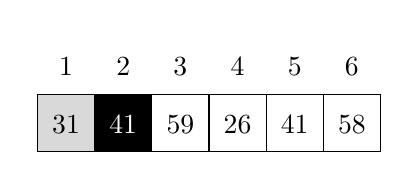
\begin{tikzpicture}[>=latex]
            \tikzstyle{row 2 column 1} = [nodes={fill=gray!30}]
            \tikzstyle{row 2 column 2} = [nodes={fill=black},text=white]
            \matrix[mymat,anchor=west,row 2/.style={nodes=draw}]
            {
                1  & 2  & 3  & 4  & 5  & 6 \\
                31 & 41 & 59 & 26 & 41 & 58 \\
            };
        \end{tikzpicture}
    \item[(b)]
        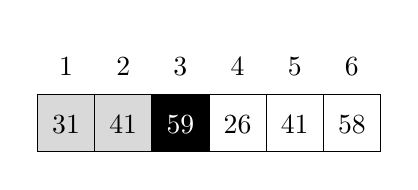
\begin{tikzpicture}[>=latex]
            \tikzstyle{row 2 column 1} = [nodes={fill=gray!30}]
            \tikzstyle{row 2 column 2} = [nodes={fill=gray!30}]
            \tikzstyle{row 2 column 3} = [nodes={fill=black},text=white]
            \matrix[mymat,anchor=west,row 2/.style={nodes=draw}]
            {
                1  & 2  & 3  & 4  & 5  & 6 \\
                31 & 41 & 59 & 26 & 41 & 58 \\
            };
        \end{tikzpicture}
    \item[(c)]
        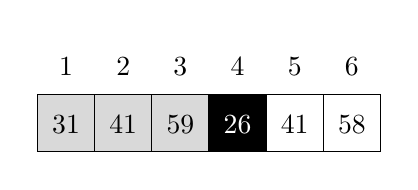
\begin{tikzpicture}[>=latex]
            \tikzstyle{row 2 column 1} = [nodes={fill=gray!30}]
            \tikzstyle{row 2 column 2} = [nodes={fill=gray!30}]
            \tikzstyle{row 2 column 3} = [nodes={fill=gray!30}]
            \tikzstyle{row 2 column 4} = [nodes={fill=black},text=white]
            \matrix[mymat,anchor=west,row 2/.style={nodes=draw}]
            {
                1  & 2  & 3  & 4  & 5  & 6 \\
                31 & 41 & 59 & 26 & 41 & 58 \\
            };
        \end{tikzpicture}
    \item[(d)]
        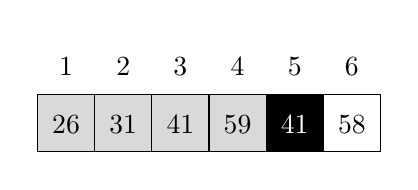
\begin{tikzpicture}[>=latex]
            \tikzstyle{row 2 column 1} = [nodes={fill=gray!30}]
            \tikzstyle{row 2 column 2} = [nodes={fill=gray!30}]
            \tikzstyle{row 2 column 3} = [nodes={fill=gray!30}]
            \tikzstyle{row 2 column 4} = [nodes={fill=gray!30}]
            \tikzstyle{row 2 column 5} = [nodes={fill=black},text=white]
            \matrix[mymat,anchor=west,row 2/.style={nodes=draw}]
            {
                1  & 2  & 3  & 4  & 5  & 6 \\
                26 & 31 & 41 & 59 & 41 & 58 \\
            };
        \end{tikzpicture}
    \item[(e)]
        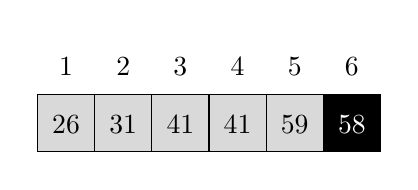
\begin{tikzpicture}[>=latex]
            \tikzstyle{row 2 column 1} = [nodes={fill=gray!30}]
            \tikzstyle{row 2 column 2} = [nodes={fill=gray!30}]
            \tikzstyle{row 2 column 3} = [nodes={fill=gray!30}]
            \tikzstyle{row 2 column 4} = [nodes={fill=gray!30}]
            \tikzstyle{row 2 column 5} = [nodes={fill=gray!30}]
            \tikzstyle{row 2 column 6} = [nodes={fill=black},text=white]
            \matrix[mymat,anchor=west,row 2/.style={nodes=draw}]
            at (0,0)
            (mat1)
            {
                1  & 2  & 3  & 4  & 5  & 6 \\
                26 & 31 & 41 & 41 & 59 & 58 \\
            };
        \end{tikzpicture}
    \item[(f)]
        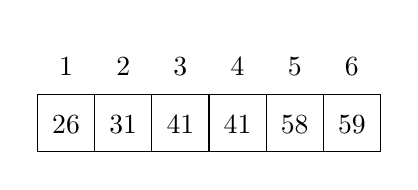
\begin{tikzpicture}[>=latex]
            \matrix[mymat,anchor=west,row 2/.style={nodes=draw}]
            at (0,0)
            (mat1)
            {
                1  & 2  & 3  & 4  & 5  & 6 \\
                26 & 31 & 41 & 41 & 58 & 59 \\
            };
        \end{tikzpicture}
\end{itemize}


\subsubsection*{2.1-2}
% Exercise 2.1-2

\begin{algorithmic}[1]
    \TITLE{\textsc{Insertion-Sort}$(A)$}
    \FOR{$j = 2$ \TO $A.\mathit{length}$}
            \STATE $\mathit{key} = A[j]$
            \STATE \COMMENT{Insert $A[j]$ to the sorted sequence $A[1\, .\, .\, j - 1]$}
            \STATE $i = j-1$
        \WHILE{$i>0$ \AND $A[i] < key$}
            \STATE $A[i+1]= A[i]$
            \STATE $i = i-1$
        \ENDWHILE
            \STATE $A[i+1] = \mathit{key}$
    \ENDFOR
\end{algorithmic}

The implementation can be seen in the following file:

\path{rs/clrs_algorithms/src/sorting.rs}.


\subsubsection*{2.1-3}
% Exercise 2.1-3

\begin{algorithmic}[1]
    \TITLE{\textsc{Linear-Search}$(A, \nu)$}
    \STATE $j = 1$
    \WHILE{$j \neq A.\mathit{length}$}
        \IF{$A[j] == \nu$}
            \RETURN $j$
        \ELSE
            \STATE $j = j + 1$
        \ENDIF
    \ENDWHILE
    \RETURN \textrm{NIL}
\end{algorithmic}

\begin{description}
    \item[Initialization:] With the loop invariant being that $A[j]$ refers to an 
        element of the sequence $A = \langle a_1, a_2, \ldots, a_n \rangle$ and 
        each element in $A[1\, .\, .\, j - 1]$ has been checked for equality, we 
        have the loop invariant valid, since $j = 1$ and $A[1]$ is in $A$ for 
        $n \ge 1$, at the start of the \textbf{while} loop 1 -- 6.
    \item[Maintenance:] Either the \textbf{if} statement in line 3 returns $A[j]$
        or the \textbf{else} statement in line 5 increments $j$ by 1, so that after
        each pass of the \textbf{while} loop, we have checked whether or not 
        $A[j] = \nu$, and the condition of the \textbf{while} loop ensures that 
        $A[j]$ is in $A$.
    \item[Termination:] If the \textbf{while} loop terminates, then either the 
        \textbf{if} condition in line 3 is true, so that $A[j] = \nu$ or 
        $j = A.\mathit{length}$, at which point we return the special value
        \textrm{NIL}.
\end{description}

Thus the algorithm is correct, since the loop invariant is initialized and 
maintained throughout, and the algorithm terminates with the correct output;
if a value is returned, $\nu$ is in $A$, and occurs at $A[j]$ for return value
$j$, otherwise the special value \textrm{NIL} was returned, and $\nu$ is not in $A$.

The implementation can be seen in the following file:

\path{src/algorithms/search/linear_search.h}.


\subsubsection*{2.1-4}
% Exercise 2.1-4

We have the following addition problem:

\begin{itemize}
    \item[\textbf{Input:}] Two $n$-element arrays $A$ and $B$ containing binary digits.
    \item[\textbf{Output:}] $(n+1)$-element array $C$ containing the sum of $A$ and $B$.
\end{itemize}

We have the following algorithm as a solution:

\begin{algorithmic}[1]
    \TITLE{\textsc{Binary-Addition}$(A, B, n)$}
    \STATE $\mathit{carry} = 0$
    \FOR{$i=1$ \TO $n$}
        \IF{$A[i] = 1$ and $B[i] = 1$}
            \IF{$\mathit{carry} == 0$}
                \STATE $C[i] = 0$
                \STATE $\mathit{carry} = 1$
            \ELSE
                \STATE $C[i] = 1$
                \STATE $\mathit{carry} = 1$
            \ENDIF
        \ELSIF{$A[i] == 1$ and $B[i] == 0$ or \\
                \qquad $A[i] == 0$ and $B[i] == 1$}
            \IF{$\mathit{carry} == 0$} 
                \STATE $C[i] = 1$
            \ELSE
                \STATE $C[i] = 0$
                \STATE $\mathit{carry} = 1$
            \ENDIF
        \ELSE
            \STATE $C[i] = \mathit{carry}$
            \STATE $\mathit{carry} = 0$
        \ENDIF
    \ENDFOR
    \STATE $C[n + 1] = \mathit{carry}$
    \RETURN $C$
\end{algorithmic}

The implementation can be seen in the following file:

\path{src/algorithms/binary/binary_addtion.h}.




\end{document}
